\chapter{SMTP, IMAP szerver}

\section{hMailServer}
\begin{flushleft}
    Be kell kapcsolni az SMTP, IMAP protokollokat, ezután meg kell adni a megfelelő domain nevét: \verb|oemail.io|. Itt hozhatunk létre IMAP fiókokat is, amit az \verb|Accounts| menüpontban tehetünk meg.
    \begin{center}
        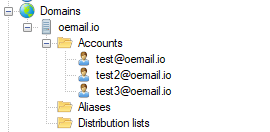
\includegraphics[width=0.5\textwidth]{hmailServer-accounts.png}
    \end{center}
\end{flushleft}

\section{Tesztelés}
\begin{flushleft}
    Megtalálható egy-egy teszt kliens, melyben kipróbálható az email szerver, amivel ellenőrizni tudjuk, hogy valóban elküldte az adott emailt a feladó és azt a vevő meg is kapta-e.
\end{flushleft}